23. \begin{figure}[ht!]
\center{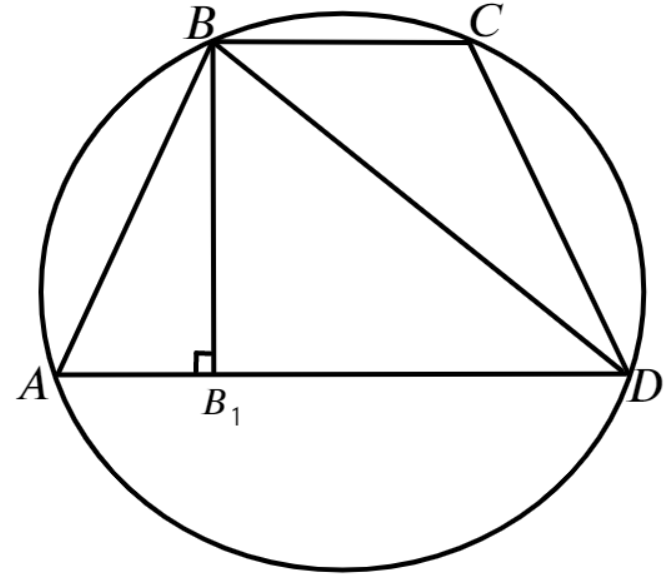
\includegraphics[scale=0.35]{g9-22.png}}
\end{figure}\\
Если трапеция является вписанной, то она равнобедренная. Если трапеция является описанной, то суммы её противоположных сторон равны, значит боковая сторона трапеции равна $\cfrac{4+16}{2}=10$см. Опустим высоту $BB_1,$ тогда $AB_1=\cfrac{16-4}{2}=6$см и $BB_1=\sqrt{100-36}=8$см. Высота трапеции равна диаметру вписанной окружности, значит её радиус равен $8:2=4$см. Описанная окружность этой трапеции является также и описанной окружностью треугольника $ABD.$ Найдём $B_1D=16-6=10$см, $BD=\sqrt{100+64}=2\sqrt{41}$см. Из треугольника $ABB_1$ имеем $\sin(\angle A)=\cfrac{8}{10}=\cfrac{4}{5},$ тогда по теореме синусов для треугольника $ABD$ получим $2R=\cfrac{2\sqrt{41}}{\cfrac{4}{5}}=\cfrac{5\sqrt{41}}{2},\ R=\cfrac{5\sqrt{41}}{4}$см.\\
